%!tex root = ../report.tex

\section{Pattern Based Reengineering}
\textbf{When to reengineer?}\\
\begin{figure}[H]
  \centering
  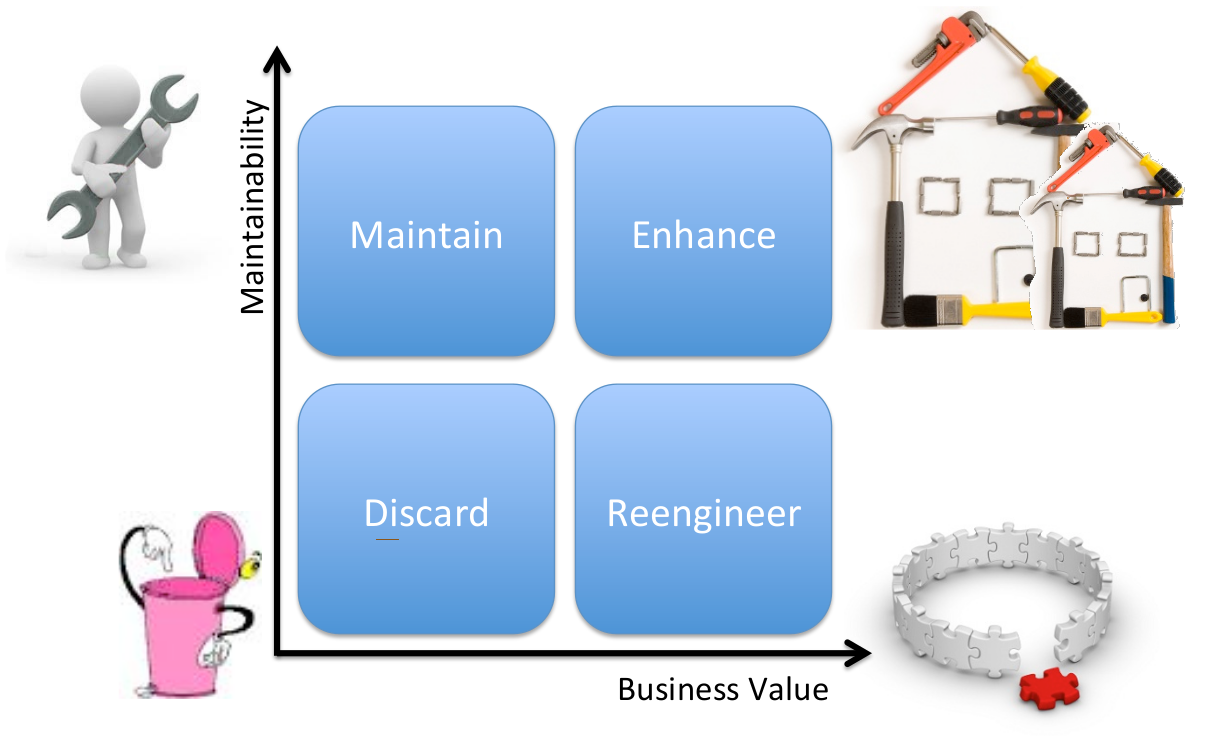
\includegraphics[width=.75\linewidth]{images/reengineering_when.png}\\
  \caption{When to reengineer?}
\end{figure}

\textbf{Reengineering Process:}
\begin{itemize}
  \item Inventory Analysis (documentation, source code, identify antipattern and smells)\
  \item Refactoring (write tests, source code refactoring)
  \item Analysis (system model, taxonomy)
  \item Object Design (object design, pattern)
  \item System Design (architectural styles)
\end{itemize}

\textbf{Refactoring:}\\
Refactoring is the process of incrementally changing the bad structure of a system or organization int a better structure.
The functionality is not changed.\\
Rules:
\begin{itemize}
  \item Small, locale and testable steps
  \item Only refactor with automated tests
  \item Test changes
  \item Finish refactoring steps before beginning new ones
\end{itemize}

\textbf{Rule of 7+-2:}\\
If an element consists of more than 7+-2 elements, there is a high chance that there is a problem (methods < 30 lines (from rule of 30), class < 7+-2 methods, package < 7+-2 classes, subsystem < 7+-2 packages)
\newpage

